Проверку \dut \ на соответствие \ref{t_capacity} настоящих~ТУ производят следующим образом:
%
\begin{enumerate}
	\item\label{itm:cap1} \dut \ заряжают согласно \ref{m_charge};
	\item\label{itm:cap2} \dut \ выдерживают при нормальной температуре окружающей среды не менее $2$~ч;
	\item\label{itm:cap3} собирают схему проверки в соответствии с рисунком~\ref{fig:capacity}, не соединяя жгут~\ref{d:cable} cо Стендом нагрузочным~\ref{d:stend};
%
		\begin{figure}[!htb]
			\centering
			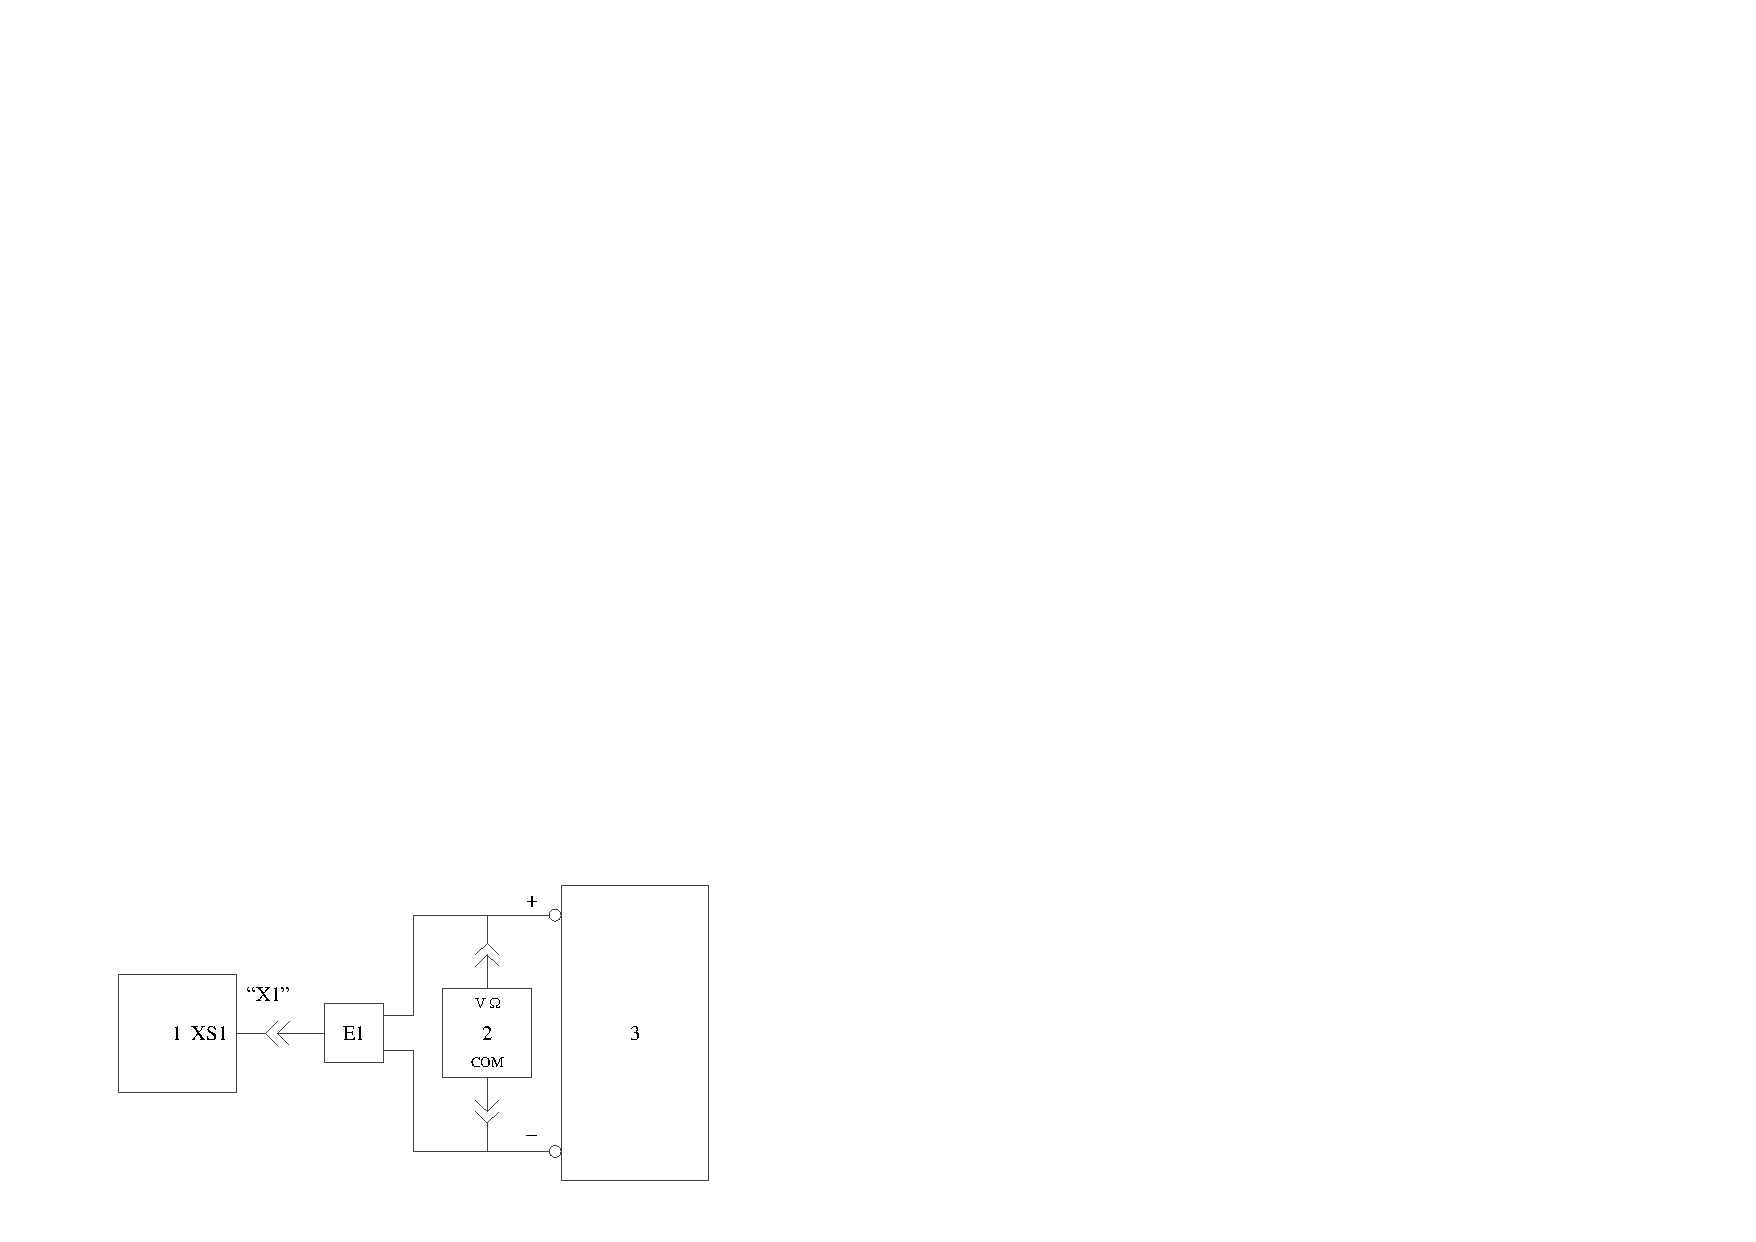
\includegraphics[page=1]{schema}
			\begin{picdescription}
				\item \ESKDtheTitle \ \RN;
				\item\label{d:multimeter} \hyperref[e:multimeter]{Мультиметр \multimeter};
				\item\label{d:stend} \hyperref[e:stend]{\stend \ \stendRN};
			\end{picdescription}
			\begin{picdescription}[label={E\arabic* ---}, ref={E\arabic*}, before={\vspace{0pt}\small}]
				\item\label{d:cable} \hyperref[e:cable]{Жгут \cableRN}.
			\end{picdescription}
			\caption{Схема проверки номинальной ёмкости, номинального напряжения, автоматической защиты от глубокого разряда в нормальных условиях}
			\label{fig:capacity}
		\end{figure}
%
	\item\label{itm:cap4} средства измерения подготавливают к работе согласно прилагаемым к ним инструкциям по эксплуатации; 
	\item\label{itm:cap5} переключают мультиметр~\ref{d:multimeter} в режим измерения сопротивления;
	\item\label{itm:cap6} измеряют сопротивление Стенда нагрузочного~\ref{d:stend} и продолжают проверку, если сопротивление составляет~$(R_{\text{н}} \pm 0,25)$~Ом, где номинальное сопротивление нагрузки~\load ;
	\item\label{itm:cap7} соединяют жгут~\ref{d:cable} со Стендом нагрузочным~\ref{d:stend};
	\item\label{itm:cap8} переключают мультиметр~\ref{d:multimeter} в режим измерения напряжения;
	\item\label{itm:cap9} измеряют исходное значение напряжения $U$ с помощью мультиметра~\ref{d:multimeter};
	\item измеряют напряжение $U_i$ каждые $\Delta t = (60 \pm 5)$~мин до снижения напряжения $U_i$ до значения ($21,0 \pm 0,5$)~В;
	\item рассчитывают ёмкость \dut \ по формуле~\eqref{eq:capacity}:
		\begin{equation}\label{eq:capacity}
			C = \sum_{i=1}^{n} \frac{U_i}{R_\text{н}},
		\end{equation}
		где $i$ "--- номер измерения, $n$ "--- количество измерений.
\end{enumerate}
 
\dut \ считают выдержавшим проверку по \ref{t_capacity} настоящих~ТУ, если рассчитанное во время испытания значение ёмкости соответствует указанному в \ref{t_capacity}.